%\documentstyle[epsf,twocolumn]{jarticle}       %LaTeX2e仕様
\documentclass[twocolumn]{jarticle}     %pLaTeX2e仕様(platex.exeの場合)
% \documentclass[onecolumn]{ujarticle}   %pLaTeX2e仕様(uplatex.exeの場合)
%%%%%%%%%%%%%%%%%%%%%%%%%%%%%%%%%%%%%%%%%%%%%%%%%%%%%%%%%%%%%%
%%
%%  基本バージョン
%%
%%%%%%%%%%%%%%%%%%%%%%%%%%%%%%%%%%%%%%%%%%%%%%%%%%%%%%%%%%%%%%%%
\setlength{\topmargin}{-45pt}
%\setlength{\oddsidemargin}{0cm}
\setlength{\oddsidemargin}{-7.5mm}
%\setlength{\evensidemargin}{0cm}
\setlength{\textheight}{24.1cm}
%setlength{\textheight}{25cm}
\setlength{\textwidth}{17.4cm}
%\setlength{\textwidth}{172mm}
\setlength{\columnsep}{11mm}

%\kanjiskip=.07zw plus.5pt minus.5pt


% 【節が変わるごとに (1.1)(1.2) … (2.1)(2.2) と数式番号をつけるとき】
%\makeatletter
%\renewcommand{\theequation}{%
%\thesection.\arabic{equation}} %\@addtoreset{equation}{section}
%\makeatother

%\renewcommand{\arraystretch}{0.95} 行間の設定
%%%%%%%%%%%%%%%%%%%%%%%%%%%%%%%%%%%%%%%%%%%%%%%%%%%%%%%%
%\usepackage{graphicx}   %pLaTeX2e仕様(\documentstyle ->\documentclass)
\usepackage[dvipdfmx]{graphicx}
\usepackage{subcaption}
\usepackage{multirow}
\usepackage{amsmath}
\usepackage{url}
\usepackage{ulem}
\usepackage{algorithm}
\usepackage{algorithmic}
\usepackage{listings} %,jlisting} %日本語のコメントアウトをする場合jlistingが必要
%ここからソースコードの表示に関する設定
\lstset{
  basicstyle={\ttfamily},
  identifierstyle={\small},
  commentstyle={\smallitshape},
  keywordstyle={\small\bfseries},
  ndkeywordstyle={\small},
  stringstyle={\small\ttfamily},
  frame={tb},
  breaklines=true,
  columns=[l]{fullflexible},
  numbers=left,
  xrightmargin=0zw,
  xleftmargin=3zw,
  numberstyle={\scriptsize},
  stepnumber=1,
  numbersep=1zw,
  lineskip=-0.5ex
}
%%%%%%%%%%%%%%%%%%%%%%%%%%%%%%%%%%%%%%%%%%%%%%%%%%%%%%%%
\begin{document}

	%bibtex用の設定
	%\bibliographystyle{ujarticle}

	\twocolumn[
		\noindent
		\hspace{1em}
		2020 年 6 月 12 日
		ゼミ資料
		\hfill
		B4 杉山 竜弥
		\vspace{2mm}

		\hrule
		\begin{center}
			{\Large \bf 進捗報告}
		\end{center}
		\hrule
		\vspace{9mm}
	]

	% ‚ここから 文章 Start!
\section{今週やったこと}
\begin{itemize}
	\item {5クラス識別を組み合わせたモデルの構築}
\end{itemize}


\section{モデルの構築}
5クラス識別を組み合わせたモデルの構築.

\begin{table}[tb]
  \begin{center}
    \caption{実験の設定}
    \begin{tabular}{|c|c|} \hline
      dataset & cifar10 \\
      data N & 2,000 / model \\ \hline
      task & 5, 10クラス識別 \\
      input & image(3x32x32) \\
      output & class(5 or 10) \\ \hline
      model & CNN(16層) \\
      optim & SDG (lr=0.001, moment=0.9) \\
      loss & Cross Entropy Loss \\ \hline
      batch size & 16 \\
      epoch & 100 \\ \hline
    \end{tabular}
    \label{tab:setting}
  \end{center}
\end{table}


\begin{figure*}[t]
	\begin{center}
		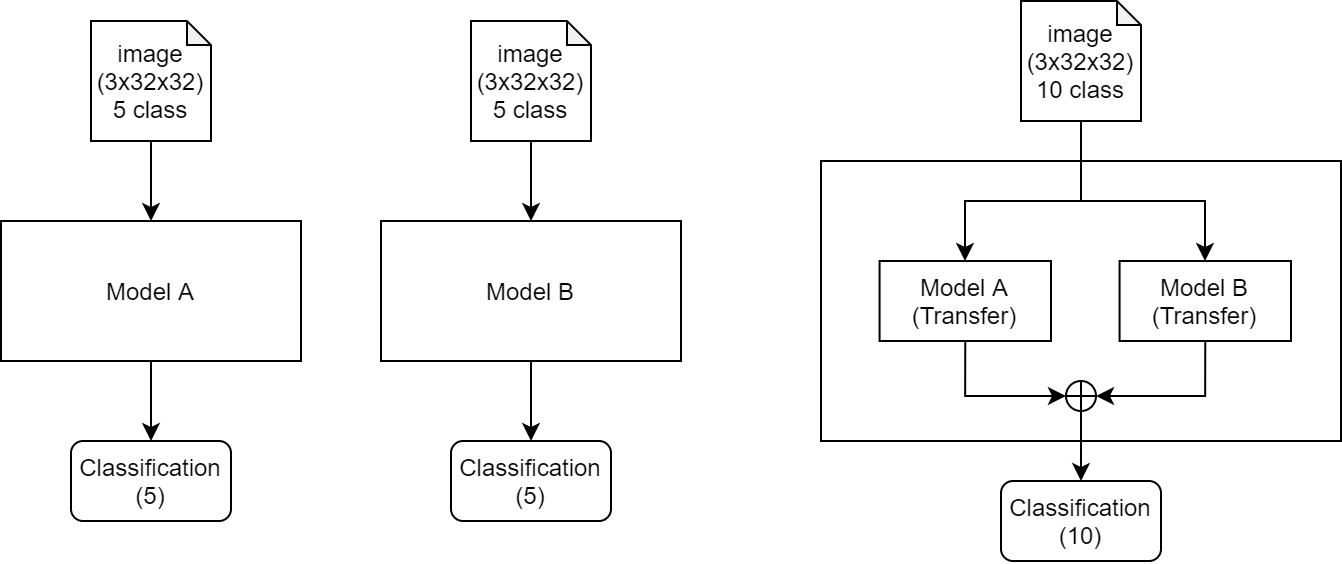
\includegraphics[clip,width=16cm]{model_figure.png}
		\caption{モデルの簡略図 ()内はデータの次元数}
		\label{fig:model}
	\end{center}
\end{figure*}

cifar10に含まれる10クラスを5クラスずつに分割した。今回はインデックスの前半(airplane, mobile, bird, cat, deer)と後半(dog, frog, horse, ship, truck)で分けることにした。生成した部分データセットを、それぞれモデルA, Bで学習した。5クラス分類ができるモデルA, Bを持つ結合モデルA + Bを作成し、10クラス分類の精度を計測した。このモデルの学習と相互関係を図\ref{fig:model}に示した。

結合モデルA + Bは10クラスのデータセットをA, Bに入力し、得られた出力をクラスインデックス順に結合して、出力とする。結合では特別な処理を行わず、そのままのデータを連結した.

\subsection{結果}

\begin{figure*}[tb]
	\begin{center}
		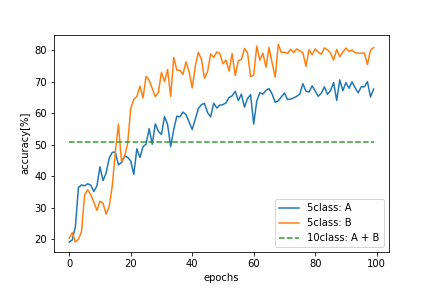
\includegraphics[clip,width=12cm]{accuracy.png}
		\caption{テストの精度の比較}
		\label{fig:accuracy}
	\end{center}
\end{figure*}

実験の結果は図\ref{fig:accuracy}にテスト精度として示した。5クラス識別ではモデルA, Bともにベースラインから始まり、Aは80\%, Bは70\%程度という精度になった. 1回の実験かつデータ数が2000であったため、同様の条件でも差が出たことが考えられる。モデルBを再度学習してみると, 80\%程度になることを後で確認した.
10クラス識別では, ベースライン10\%に対して, 50\%という結果となった. さらに精度を高めるには、結合方法の改良が必要と考えられる。

\section{考察}
% 精度が出ない,とかだけではなく自分なりの考察を示す
クラスの分割パターンを変えて、実験

モデルの結合方法の調査

\section{今後の予定}
% なんとなくなんかの勉強をするとかではなく具体的に
\begin{itemize}
	\item {モデルの完成と実験}
\end{itemize}

% 参考文献リスト
\bibliographystyle{unsrt}
\bibliography{ref}
\end{document}
